% To be used for generating only 1 chapter of the thesis

\title{Side-Channel Security in Networks: From the Internet to Interconnects}

\author{Rut Vora}
\previousdegree{B. Engineering in Computer Science, BITS-Pilani, 2020}


\degreetitle{Master of Science}

\institution{The University of British Columbia}
\campus{Vancouver}

\faculty{The Faculty of Graduate and Postdoctoral Studies}
\department{Computer Science}
\submissionmonth{March}
\submissionyear{2025}

\examiningcommittee{Aastha Mehta, Assistant Professor, Computer Science, \textsc{UBC}}{Supervisor}
% \examiningcommittee{Mathias L\'{e}cuyer, Assistant Professor, Computer Science, \textsc{UBC}}{Co-Supervisor}
% \examiningcommittee{Margo Seltzer, Professor, Computer Science, \textsc{UBC}}{Supervisory Committee Member}

%% hyperref package provides support for embedding meta-data in .PDF
%% files
\hypersetup{
  pdftitle={Side-Channel Security in Networks: From the Internet to Interconnects  (DRAFT: \today)},
  pdfauthor={Rut Vora},
  pdfkeywords={PCIe, CXL, Side Channels, Networks, Proxy}
}

\begin{document}

\maketitle

\textspacing		% begin one-half or double spacing

% Body of Thesis (not all sections may apply)
\mainmatter

\acresetall	% reset all acronyms used so far

% Main Sections
\chapter{NetShaper: A Differentially-Private Side Channel Mitigation System}

NetShaper \cite{sabzi2024netshaper} is both the name of the framework and the system that implements the framework to mitigate network side-channel attacks in internet applications.
We have provided a brief outline of the framework in \Cref{sec:netshaper-framework-bg}. 
Here, we describe the NetShaper system.

We first outline the requirements that the system should fulfil.
First, in any given window $W$, the system should be able to obtain the size of the payload in the buffering queue, with noise added to it. 
That is, the system should be able to complete the execution of $f_{DP}(S, t_{start}, t_{start} + W)$.
In the same window, the system should also be able to send out the payload, with padding, if necessary, such that the total data sent out, $b_{out}$, is equal to the noised size. 
However, it is sufficient to be able to queue $b_{out}$ bytes to be sent out, even if the actual transmission goes beyond the window $W$, as long as any delays were not caused by the payload coming in or already present in the buffering queue. 
The reason for this is the post-processing property of DP that we outlined in \Cref{subsec:dp-bg}.

Second, the payload and the padding should be indistinguishable to any observer observing the outbound packet stream.
Hence, the payload and padding should both be subject to the same congestion control, re-transmission, loss recovery, and other network behaviour.
In addition, the outbound transmission should provide the same or a higher level of reliability than the applications using this system expect.

Finally, the system should be modular so that modifications to any one sub-component do not require changes in the other components.
The system should also be portable and easily deployable, requiring none to minimal changes on the end hosts where the applications are running.
These goals ascertain that the system is easy to adopt and deploy and can easily be modified per the deployer's requirements.


% 1. Complete DP measurement within the window W
% 2. Data and Dummy should be indistinguishable
% 3. Should provide the same level of reliability the application expects
% 4. Should be modular for easy modification to sub-components
% 5. Should be portable and easily deployable, with minimal modifications of the end-hosts.

\section{Proxy Architecture}
\label{sec:proxy-arch}

\begin{figure}[!htb]
    \centering
    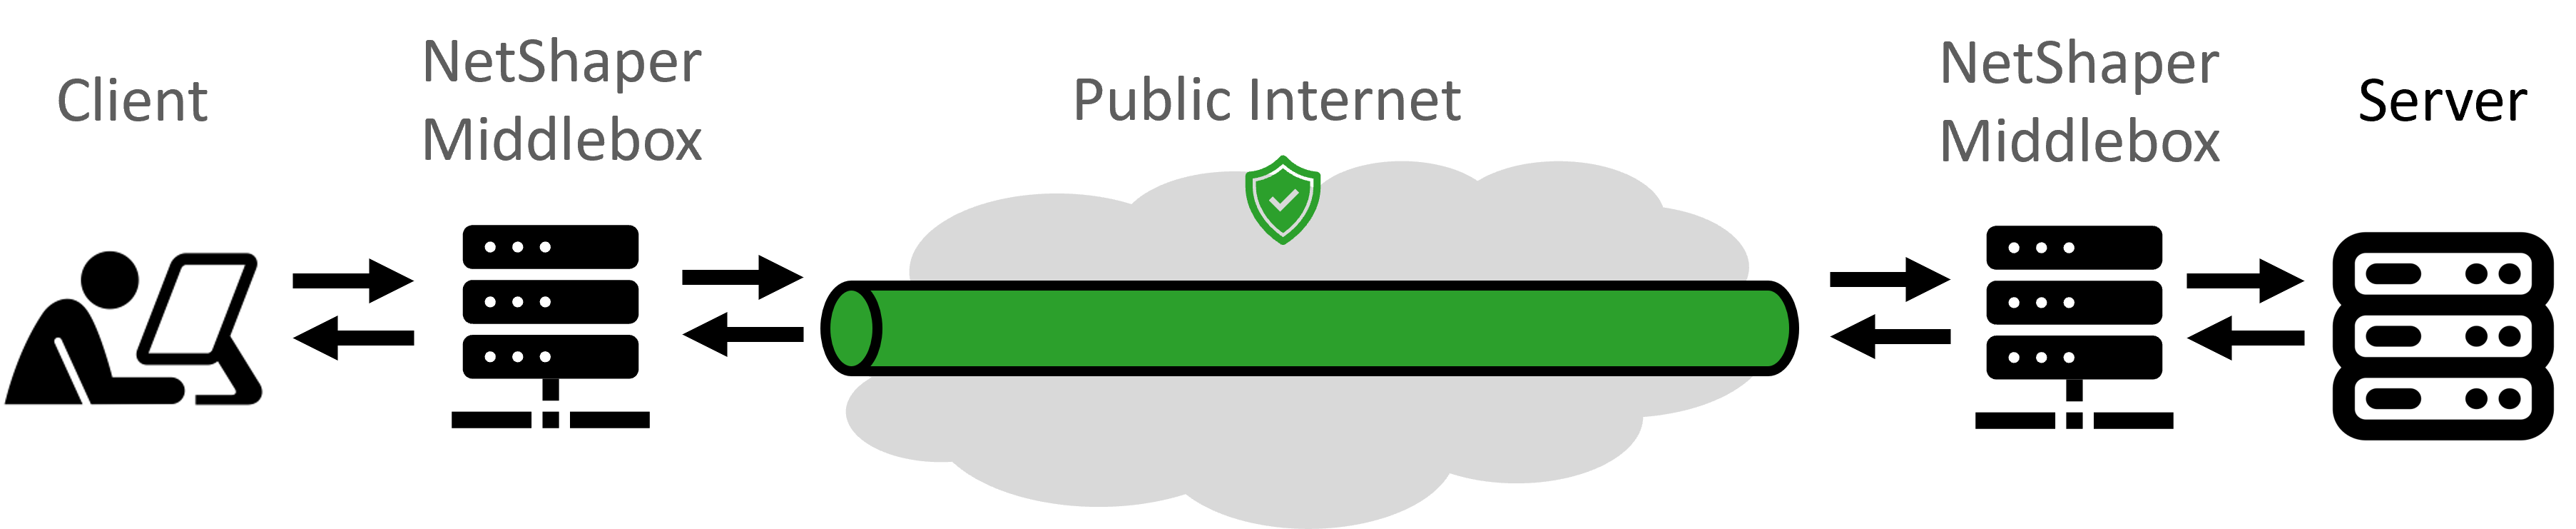
\includegraphics[width=\columnwidth]{figures/netshaper/netshaper-setup.png}
    \caption{NetShaper's Tunnel Setup}
    \label{fig:netshaper-setup}
\end{figure}

We designed NetShaper as a modular system that can be deployed using a pair of middleboxes, forming a forward and reverse proxy pair (see \Cref{fig:netshaper-setup}). 
Here, we describe in detail the architecture of the proxy setup and defer the discussion regarding the design of the middlebox to \Cref{sec:mb-design}. 

When using NetShaper, all clients communicate with the servers using three piecewise connections: 
(\textit{i}) between the client and the client-side middlebox, 
(\textit{ii}) between the client-side middlebox and the server-side middlebox, and
(\textit{iii}) between the server-side middlebox and the server.

For connection \textit{i} and \textit{iii}, NetShaper relies on standard TCP/UDP protocols. However, for connection \textit{ii} (i.e. to proxy the payload), NetShaper utilises QUIC. 
Using QUIC to proxy the payload avoids the TCP meltdown problem [??] that occurs when tunnelling TCP via TCP.
In addition, using QUIC also avoids the problem of an observer/attacker being able to distinguish between payload and padding that would occur when TCP was tunnelled via UDP (as the end host would retransmit payload, but the padding would not be retransmitted).

\paragraph{Setup.}
In order to be able to proxy end host traffic via NetShaper, the middleboxes need to be configured. 
The middleboxes first establish an encrypted QUIC connection between them, with user-specified reliability semantics.
Once the QUIC connection is established, NetShaper initialises three types of QUIC streams: Control, Data (Payload), and Dummy (Padding).
One \textit{control} stream is used to transmit messages regarding connection establishment or termination by the end host.
One \textit{dummy} stream is used for adding padding to the payload whenever necessary, based on the output of $f_{DP}$
\footnote{We avoid the use of PADDING frames in QUIC as they do not elicit acknowledgements and hence are distinguishable from the payload \cite{quic_rfc}.}.

\paragraph{Supporting multiple end hosts.}
As we discussed in \Cref{sec:quic-bg}, QUIC supports multiple streams in the same connection.
Using this, NetShaper can proxy the payload of multiple end hosts through a single QUIC connection between a pair of middleboxes.

While QUIC can support arbitrary initialisation and termination of streams, each stream has an associated header, which would increase the total transmission size.
For example, when transmitting two bytes in a single stream, the total transmission size would be $2 + S_{header}$.
However, when transmitting two streams of one byte each, the total transmission size would be $2 + 2*S_{header}$. 
An adversary may be able to distinguish between these two scenarios.
In order to avoid such a situation, NetShaper fixes and initialises a fixed number of streams per QUIC connection during the setup phase.
NetShaper assigns an unused stream to the client whenever a new client connects to the middlebox.
Similarly, NetShaper marks a stream as unused when an end host terminates the connection.

\endinput
\section{Middlebox Design}
\label{sec:mb-design}

While it is possible to apply NetShaper framework's approach at any network layer, we chose to develop the system as an L4 (Transport Layer) proxy.
This enables the system to be easily deployable, entirely in userspace and without requiring any superuser privileges. 
Developing NetShaper at L2 (Data Link Layer) or L3 (Network Layer) would require the deployer to either have the ability to modify the OS kernel or deploy some form of kernel bypass.

\begin{figure}[!htb]
    \centering
    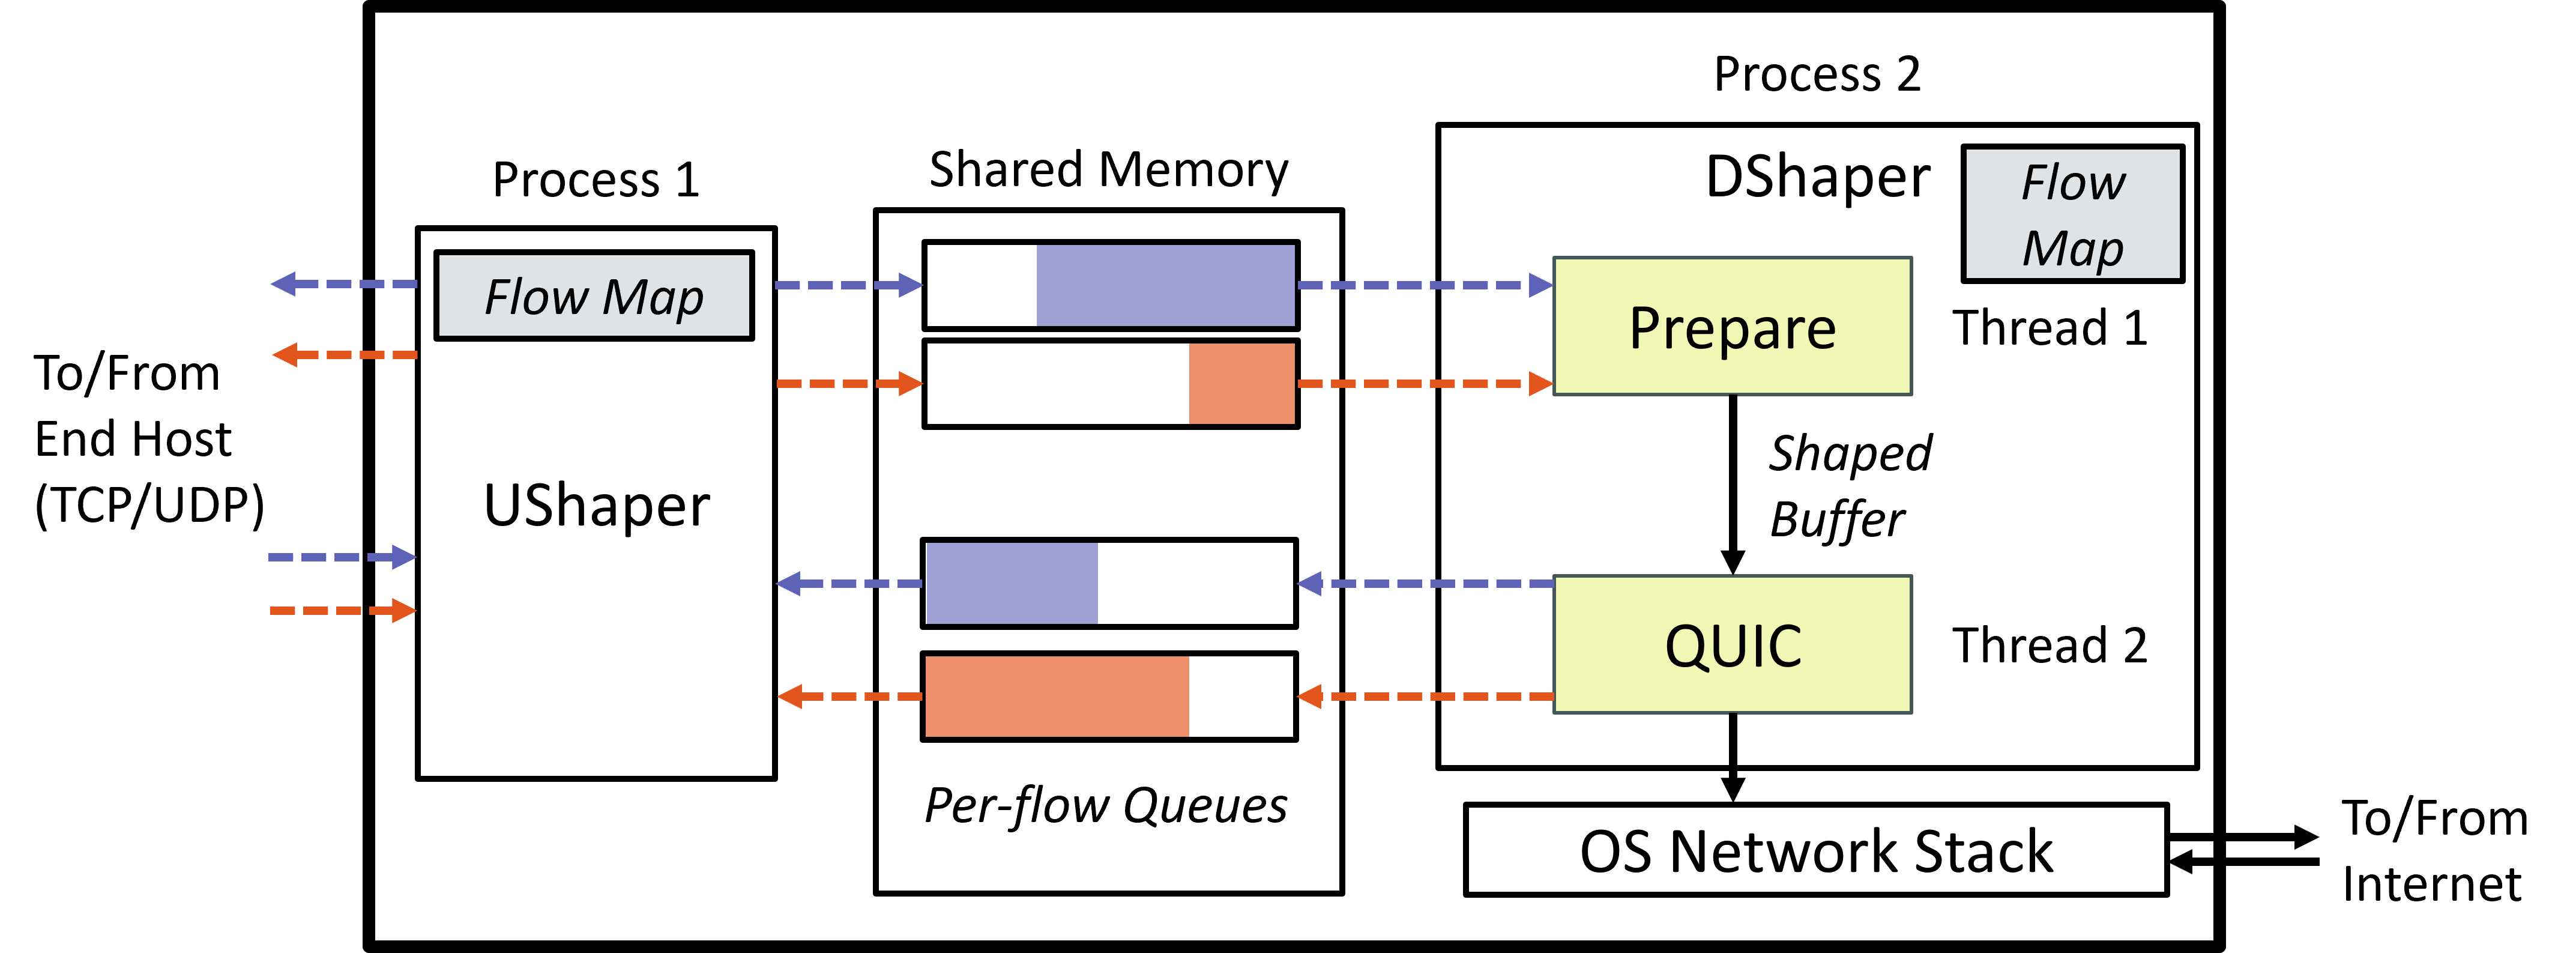
\includegraphics[width=\columnwidth]{figures/netshaper/middlebox-design.png}
    \caption{NetShaper Middlebox Design}
    \label{fig:middlebox-design}
\end{figure}

As outlined in \Cref{fig:middlebox-design}, NetShaper's middlebox consists of two main processes: UShaper and DShaper, and a shared memory between them.

\paragraph{UShaper.}
The \textit{UShaper} implements a client or a server to communicate with the end host.
It shares some Lamport Queues (LQs) [??] with DShaper.
It also consists of a flow map that maps a client with a corresponding pair of LQs.
\textit{UShaper} updates the flow map whenever a client establishes or terminates a connection.
In addition, it assigns an unused pair of LQs (one outbound and one inbound) to a new client and revokes that whenever the client terminates the connection.
The \textit{UShaper} receives outbound traffic from the end host and enqueues the payload in the assigned LQ.
Similarly, it dequeues inbound traffic from the inbound LQs and sends it to the corresponding end hosts.

\paragraph{DShaper.}
The \textit{DShaper} consists of two threads: \textit{Prepare} and \textit{QUIC worker}, and a flow map.
The flow map maps an LQ with a pre-initialised QUIC stream.
The \textit{Prepare} thread also measures the data available in the outbound LQs at the start of the window $W$.
It then adds noise to this available size based on the DP parameters.
Finally, it enqueues the payload and padding that needs to be transmitted.
The \textit{QUIC worker} transmits the enqueued data out to the network.
It also processes the received data, places it in the relevant LQ, and updates the flow map whenever a client initialises or terminates a connection.

In order to ensure that the operation of \textit{UShaper}, \textit{Prepare}, and \textit{QUIC worker} do not interfere with each other, we apply a few constraints in the implementation, and during the deployment of NetShaper.
First, all three components are required to be pinned on separate cores so that the execution time of one may not impact the others.
Second, in order to not leak the size of the payload due to the processing time of the enqueue operation done by the \textit{Prepare} thread, the \textit{Prepare} thread applies a lock for a fixed duration, during which the \textit{QUIC worker} can not transmit the data. 
We have outlined pseudo-code for both prepare and QUIC worker in \Cref{lst:prepare_and_worker}.
Finally, when receiving data, the \textit{QUIC worker} also enqueues the dummy bytes to a designated LQ so that the processing time remains consistent with the size of the data (see Figure ??).

\paragraph{Shared Memory.}
Both \textit{UShaper} and \textit{DShaper} have a shared memory between them.
This shared memory consists of three types of LQs: Control, Payload, Dummy
Similar to the stream types outlined in \Cref{sec:proxy-arch}, \textit{Control} LQ transmits the information about a connection establishment or termination by a client. 
\textit{Payload} LQ consists of the bytes received from the end host or to be sent to the end host.
\textit{Dummy} LQ consists of the dummy/padding bytes that are received.

\begin{minipage}{\textwidth}
\lstinputlisting[language=Python]{code/netshaper/prepare_and_worker.py}
\captionsetup{type=lstlisting}
\caption{Prepare and QUIC Worker Pseudo-code}
\label{lst:prepare_and_worker}
\end{minipage}

\endinput


\begin{figure}[!htb]
    \centering
    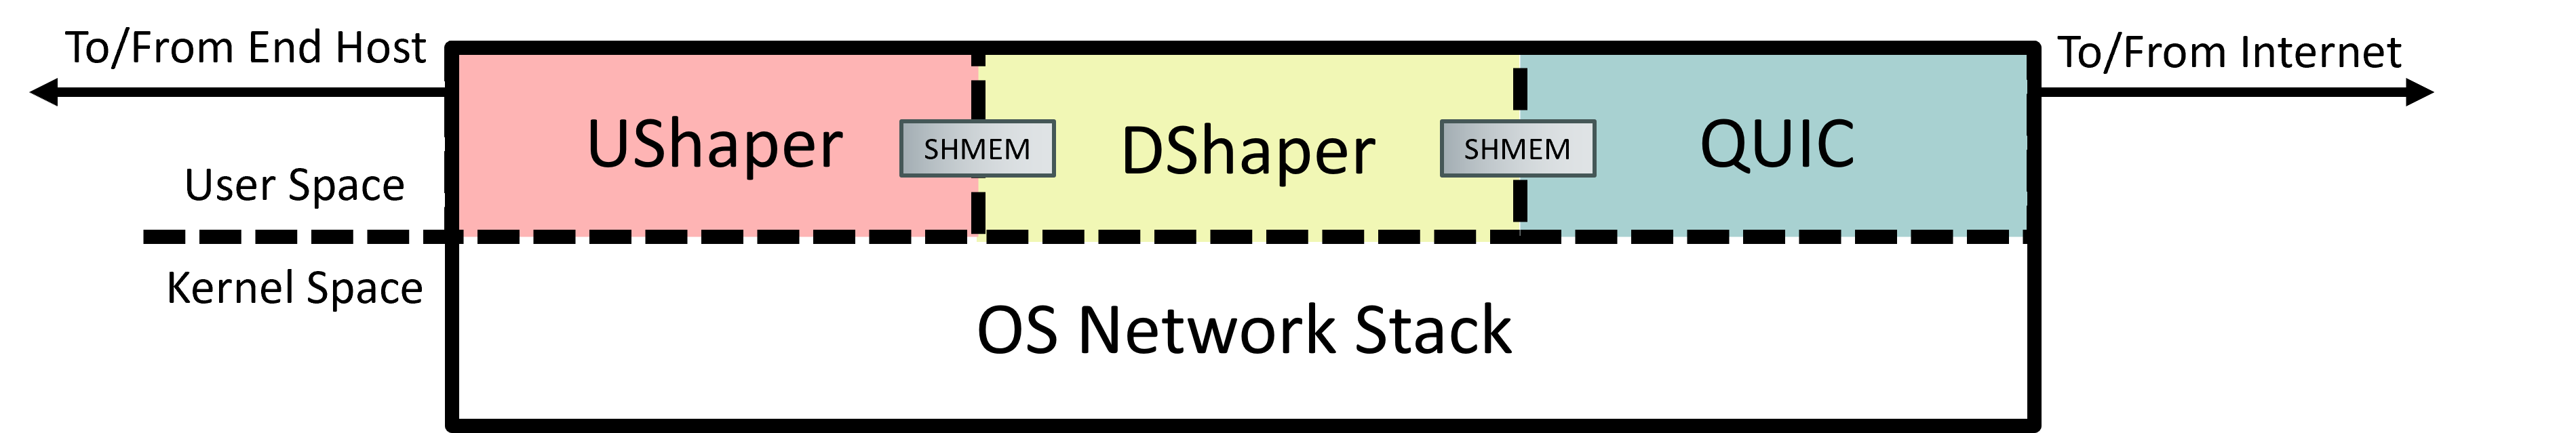
\includegraphics[width=\columnwidth]{figures/netshaper/middlebox-design-overview.png}
    \caption{Overview of NetShaper's Middlebox}
    \label{fig:middlebox-design-overview}
\end{figure}

\endinput

Should we add pseudo-codes for UShaper and DShaper?
\section{Performance}\label{sec:netshaper-performance}
\section{Limitations and Discussion}\label{sec:netshaper-discussion}

\endinput

\begin{singlespace}
\raggedright
\bibliographystyle{abbrvnat}
\bibliography{biblio}
\end{singlespace}

\end{document}
